\chapter{A Linear Kernel for Planar Semitotal Domination}\label{ch:linkern}

\vspace*{-50pt}
\begin{figure}[ht]
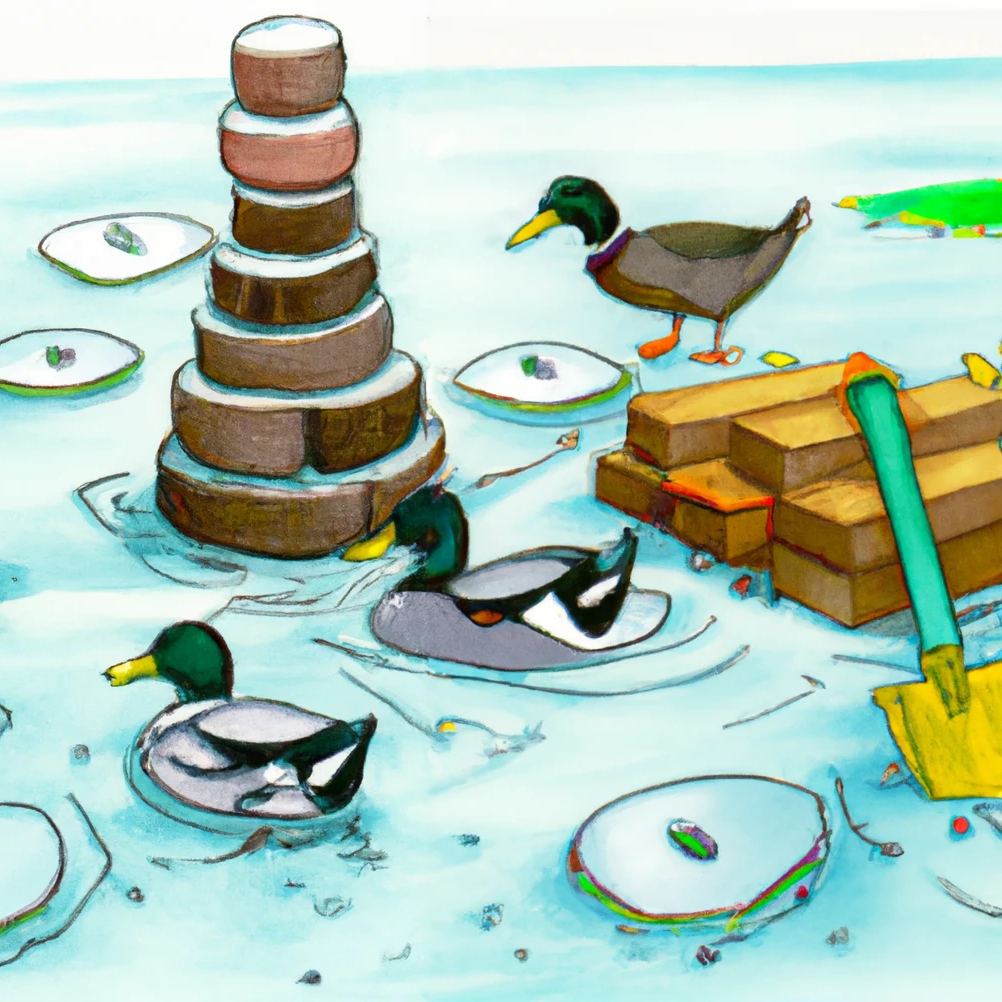
\includegraphics[width=.3\textwidth, right]{img/constructing.png}
        \captionsetup{textformat=empty,labelformat=blank}
        \caption[Generated with Dalle-E. Knowledge Cutoff 09-2022]{Generated with Dall-E. \url{https://labs.openai.com/}. ``more ducks building and working on  a high stack in the water using an excavator and tools and machines''}
\end{figure}

\epigraph{\itshape The best way to explain it is to do it.}{Lewis Caroll, \textit{Alice in Wonderland}}

We will present a polynomial-time preprocessing procedure giving a linear kernel for \psdom parameterized by solution size. Based on the technique first introduced by Alber, Fellows, and Niedermeier~\cite{Alber2004} in 2004, an abundance of similar results to other domination problems emerged which gave us the belief we can transfer these results to \sdom. 
\cref{tbl:kernels} gives an overview of the status of various kernels for the planar case on various domination problems.
All of these results introduce reduction rules bounding the number of vertices inside so-called ``regions'' which can be obtained by a decomposition of the planar graph. 

\begin{table}[h]
\begin{minipage}[th]{\linewidth}
\setcounter{mpfootnote}{\value{footnote}}
\renewcommand{\thempfootnote}{\arabic{mpfootnote}}

\begin{tabularx}{\textwidth}{lcX}
\textbf{Problem} & \textbf{Best Kernel} & \textbf{Source} \\
\pdom &  $67k$ &~\cite{Diekert2005}\footnotemark\\
\ptdom &  $410k$ &~\cite{Garnero2018}\footnotemark \\
\psdom & $\kernelsize k$ & \cref{thm:central} \\
& & \\
\peddom & $14k$  &~\cite[Th. 2]{Guo2007} \\
\pefdom &  $84k$ &~\cite[Th. 4]{Guo2007} \\
\prbdom &  $43k$ &~\cite{Garnero2017} \\
\pcdom & $130k$  &~\cite{Luo2013} \\
\pdirdom & Linear  &~\cite{Alber2006}  \\
\end{tabularx}

\footnotetext[1]{Halseth's master thesis~\cite{Halseth2016} claims a bound of $43k$, but no conference or journal version was found.}
\footnotetext[2]{Improved their own results from first $694k$~\cite[arXiv v2]{Garnero2018}}
\setcounter{footnote}{\value{mpfootnote}}
\end{minipage}
\caption{An overview about existing kernels for planar dominating problems.}
\label{tbl:kernels}
\end{table}
In the following years, this approach bore fruits for other planar problems as well:
a ${}^{11}{\mskip -5mu/\mskip -3mu}_3$ kernel for \name{Connected Vertex Cover}\xspace given in~\cite{Kowalik2013},
$624k$ for \name{Maximum Triangle Packing}\xspace,
$40k$ for \name{Induced Matching}\xspace,
$13k$ for \name{Feedback Vertex Set}\xspace and further linear kernels for
\name{Full-Degree Spanning Tree}\xspace and
\name{Cycle Packing}\xspace~\cite{Wang2011, Kanj2011, Bonamy2016, Guo2006, Garnero2019}.

In the upcoming years, this approach was generalized to larger graph classes. 
Fomin and Thilikos~\cite{Fomin2004} started by proving that the initial reduction rules in~\cite{Alber2004} can be extended to obtain a linear kernel on graphs with bounded genus $g$ for \dom.
Gutner~\cite{Gutner2009} advanced in 2008 by giving a linear kernel for $K_{3,h}$-topological-minor-free graph classes and a polynomial kernel for $K_h$-topological-minor-free graph classes. 
In 2012 Philip, Raman, and Sikdar~\cite{Philip2012} showed that $K_{i,j}$-free graph classes admit a polynomial kernel. 
In an attempt to further expand these ideas to other problems, Bodlaender et al.~\cite{Bodlaender2016} proved that all problems expressible in counting monadic second-order logic satisfying a coverability property admit a polynomial kernel on graphs of bounded genus $g$. 
Interestingly from a theoretical point of view, the constants in these meta-theorems for the kernels obtained are too large to be of practical interest. 
The question of how an efficient kernel for the \psdom problem can be constructed remains. 

In this chapter, we will transfer the linear kernel with ``reasonable'' small constants for \ptdom described by Garnero and Sau~\cite[arXiv v2]{Garnero2018} to \psdom. 
We modified the original reduction rules to preserve the witness properties of an sds. 

 \paragraph{The Main Idea} A planar graph \G with a given vertex set $D \subseteq V$ can be decomposed into at most $(3 \cdot \abs{D}-6)$ so-called ``regions'' (\cref{def:region}). 
 If $D$ is a given sds of size $\abs{D}$, the total number of regions in this decomposition depends \underline{linearly} on the size of $D$. 
 We define \textit{reduction rules} (\cref{rgl:rone,rgl:rtwo,rgl:rthree}) to iteratively reduce the number of vertices around a region.
 After, we bound the size of a resulting graph by proving that for a fixed $k$ each region has only a constant number of vertices nearby. 
Such a reduction gives us a \textit{kernel} for \psdom.

Interestingly, the reduction rules do not rely on the decomposition itself, but rather consider the neighborhood of every pair of vertices in the graph. 
The decomposition has just been used as a tool to analyze the kernel size after the reduction.


\section{Definitions}

Before stating the reduction rules, we need definitions to capture the ``nice'' properties we are to exploit. 
They are equal to those given by Garnero and Sau for \ptdom in~\cite[arXiv v2]{Garnero2018} and for \prbdom in~\cite{Garnero2017} which in turn reused ideas introduced by Alber, Fellows and Niedermeier~\cite{Alber2004} for \pdom.
The main idea is to partition the neighborhoods of both a single vertex and a pair of vertices respectively into three distinct subsets which intuitively classify how much these vertices are confined and how closely they are related to the rest of the graph.
Recall for the following definition that ${N(v) = \{u \in V : \{u,v\} \in E \}}$ and ${N[v] = N(v) \cup \{v\}}$ the closed neighborhood of a vertex $v$.

\begin{definition}
    \label{def:nv}
    Let \G be a graph and let $v \in V$. We split $N(v)$ into three subsets:
    \begin{align}
        N_1(v) & = \{u \in N(v) : N(u) \setminus N[v] \neq \emptyset \}              \\
        N_2(v) & = \{u \in N(v)\setminus N_1(v) : N(u) \cap N_1(v) \neq \emptyset \} \\
        N_3(v) & = N(v) \setminus (N_1(v) \cup N_2(v))
    \end{align}
    For $i,j \in [1,3]$, we denote $N_{i,j} (v) := N_i(v) \cup N_j(v)$. Furthermore, we call a vertex $v'$ \textit{confined} by a vertex $v$, if $N(v') \subseteq N[v]$.
\end{definition}

\begin{figure}[h]
    \label{fig:neighborhoodSingle}
    \begin{equation*}
        \tikzfig{fig/tikz/neighborhoods-single-vertex}
    \end{equation*}
   \caption[The neighbordhood of a single Vertex $v$]{\textit{The neighborhood of a single vertex v split to $N_1(v)$ ({\setulcolor{NONE}\ul{purple}}), $N_2(v)$ ({\setulcolor{NTWO}\ul{blue}}), and $N_3(v)$ ({\setulcolor{NTHREE}\ul{olive}}).
    $N_1(v)$'s are those having neighbors outside $N(v)$, $N_2(v)$'s are a buffer between $N_1(v)$ and $N_3(v)$, and $N_3(v)$-vertices are confined in $N(v)$}.}
\end{figure}

We will shortly discuss the definition of these sets:

\begin{xltabular}{\textwidth}{lX}
\textbf{$\mathbf{N_1(v)}$} & are all the neighbors of $v$ having at least one neighbor outside of $N(v)$ and connect $v$ with the rest of the graph. 
They are the only vertices with the power to dominate vertices outside the neighborhood of $v$. \\

\textbf{$\mathbf{N_2(v)}$} & contains all neighbors of $v$ not from $N_1(v)$ with at least one neighbor in $N_1(v)$. 
These vertices do not have any function as dominators and are placed in between a vertex from $N_1(v)$ and those from  $N_3(v) \cup \{ v \}$. 
They are useless as witnesses because either we can replace them with $v$ (sharing the same neighborhood) or we replace them with a $z \in N_1(v)$ if they function as a witness for $v$. \\

\textbf{$\mathbf{N_3(v)}$} & vertices are sealed off from the rest of the graph. 
They are useless as dominators: For all $z \in N_3(v)$, $N(z) \subseteq N(v)$ by definition and thus, we would always prefer $v$ as a dominating vertex instead of $z$. 
They can still be necessary as a witness for $v$ if $N_1(v) \cup N_2(v) =\emptyset$ but this can only happen if $v$ forms a connected component with only $N_3(v)$ vertices as neighbors. 
We will be using this observation in \cref{rgl:rone} to shrink $\abs{N_3(v)} \leq 1$.
\end{xltabular}

Next, we will extend this notation to a pair of vertices which we will later use in  \cref{rgl:rtwo} to reduce the neighborhood of two vertices. We will classify how strongly the joined neighborhood $N(v) \cup N(w)$ of two vertices is connected to the rest of the graph.

\begin{definition}
    Let \G be a graph and $v,w \in V$. We denote by ${N(v,w) := N(v) \cup N(w)}$ the joined neighborhood $N(v) \cup N(w)$ of the pair $v,w$ and split $N(v,w)$ into three distinct subsets:
    \begin{align}
        N_1(v,w) & = \{u \in N(v,w) \mid N(u) \setminus (N(v,w)\cup \{v,w\}) \neq \emptyset \}  \\
        N_2(v,w) & = \{u \in N(v,w)\setminus N_1(v,w) \mid N(u) \cap N_1(v,w) \neq \emptyset \} \\
        N_3(v,w) & =  N(v,w) \setminus (N_1(v,w) \cup N_2(v,w))
    \end{align}
    For $i,j \in [1,3]$, we denote $N_{i,j}(v,w) = N_i(v,w) \cup N_j(v,w)$.
\end{definition}

Similiar as before, \textbf{$\mathbf{N_1(v,w)}$} contains vertices with at least one neighbor outside $N[v] \cup N[w]$, \textbf{$\mathbf{N_2(v, w)}$}-vertices are in between those from $N_3(v,w) \cup \{v, w\}$ and $N_1(v,w)$, and \textbf{$\mathbf{N_3(v,w)}$} contains vertices isolated from the rest of the graph. 

A vertex $v \in N_i(v)$ is not necessarily also in $N_i(v,w)$! Observe the vertex $z$ in \cref{fig:neighborhoodDouble}. 
Unlike the sets $N_1(v), N_2(v)$ and $N_3(v)$, in every one of the distinct sets $N_i(v,w)$ ($i \in [3]$) there can be vertices that belong to an sds. See \cref{fig:alldominating} for examples.

\begin{figure}[]
    \begin{equation*}
        \tikzfig{fig/tikz/neighborhoods-two-vertices}
    \end{equation*}
    \caption[The neighborhood of a pair of vertices]{\textit{The neighborhood of a pair of vertices. Vertices from $N_3(v,w)$ are colored {\setulcolor{NTHREE}\ul{olive}}, $N_2(v,w)$'s {\setulcolor{NTWO}\ul{blue}} and $N_1(v,w)$'s {\setulcolor{NONE}\ul{purple}}.
    Note that $z \in N_1(w)$, because there is an edge to a neighbor of $v$, but $z \notin N_1(v,w)$ (and rather $z \in N_3(v,w)$)}.}
    \label{fig:neighborhoodDouble}
\end{figure}


\begin{figure}[]
        \begin{equation*}
            \tikzfig{fig/tikz/ntwoimportant}
    \end{equation*}
    \caption[Example for $N_2(v,w)$ dominating]{Contrary to $N_i(v)$, vertices from all $N_i(v,w)$ can be dominators. 
    Left: $\{d_1, d_2\}$ with $d_2 \in N_2(v,w)$ form the only minimum sds. Right: $d_1 \in N_1(v,w)$ and $d_2 \in N_3(v,w)$ optimal.}
    \label{fig:alldominating}
\end{figure}

\subsection{Reduced Graph}

Before stating the reduction rules, we want to clarify when we consider a graph to be \textit{reduced}. 

\begin{definition}[\cite{Garnero2017}]\label{def:reduced}
    A graph \G is \underline{reduced under} a set of rules if either none of them can be applied to $G$ or the application of any of them creates a graph isomorphic to $G$.
\end{definition}

\cref{def:reduced} differs from the definition usually used where a graph $G$ is \textit{reduced} under a set of reduction rules if none of them can be applied to G anymore (compare e.g.~\cite{Fomin2019}). Some of our reduction rules (\cref{rgl:rone} or \cref{rgl:rtwo}) could be applied \textit{ad infinitum} creating an endless loop that does not change $G$ anymore. Our definition guarantees termination in that case. 
All of the given reduction rules are local and only need the neighborhood of at most two vertices.
They are replaced partially with gadgets of constant size.  
Checking whether the application of one of the rules created an isomorphic graph can therefore be accomplished in constant time because only the neighbors of these vertices might have changed and recognizing this can already be done while each rule itself is active. 
If all rules created an isomorphic graph, we exit the reduction procedure.

\subsection{Regions in Planar Graphs}

Alber, Fellows and Niedermeier~\cite{Alber2004} gave a novel approach to look at planar graphs. In their analysis, they stated a constructive algorithm that decomposes a planar graph into local ``regions''. Intuitively, assume that we have a fixed plane embedding of a planar graph \G. If we pick two distinct vertices $v$ and $w$ from a given \sdom $D \subseteq V$ that are at most of distance two apart, we can try to find two distinct paths from $v$ to $w$ that span up the boundaries of a face and enclose as many other vertices as possible. 

The following definitions are based on those given by Garnero and Sau in~\cite[arXiv v2]{Garnero2018} and will lead towards a clean definition of a \textit{region} and what we understand as a \dreg. More detailed explanations and concrete examples can be found in their paper.

% TODO Define Contracting and clockwise order
\begin{definition}
    Two simple paths $P_1, P_2$ in a plane graph G are \underline{confluent} if at least one of the following statements holds:
    
    \begin{enumerate}
        \item they are vertex-disjoint;
        \item they are edge-disjoint and for every common vertex $u$, if $v_i, w_i$ are the neighbors of $u$ in $p_i$, for $i \in [1,2]$, it holds that $[v_1, w_1, v_2, w_2]$;
        \item they are confluent after contracting common edges.
    \end{enumerate}
\end{definition}

% TODO A picture for each of the cases

% TODO MORE TEXT HERE: GIVE MORE INTUITION
\begin{definition}
    Let \G be a plane graph and let $v,w \in V$ be two distinct vertices. A \underline{region $R(v,w)$} (also denoted as $vw$-region $R$) is a closed subset of the plane, such that:
    \begin{enumerate}
        \item the boundary of $R(v,w)$ is formed by two confluent simple $vw$-paths with length at most 3
        \item every vertex in $R(v,w)$ belongs to $N(v,w)$, and
        \item the complement of $R(v,w)$ in the plane is connected.
    \end{enumerate}
    
    The \underline{poles} of R are the vertices $v$ and $w$. 
    The boundary paths are the two $vw$-paths that form $\partial R$.
    We denote with $\partial R$ the set of vertices on the boundary of $R$ (including the poles) and by $V(R)$ the set of vertices laying (on the plane embedding) in $R$. 
    Furthermore, we call $\abs{V(R)}$ the \underline{size} of the region of the region.
    
\end{definition}

\begin{definition}
    Two regions $R_1$ and $R_2$ are non-crossing, if:
    \begin{enumerate}
        \item $(R_1 \setminus \partial R_1) \cap R_2 = (R_2 \setminus \partial R_2) \cap R_1 = \emptyset$, and
        \item the boundary paths of $R_1$ are pairwise confluent with the ones in $R_2$.
    \end{enumerate}
\end{definition}

We now have all the definitions ready to formally define a maximal \dreg on planar graphs:

\begin{definition}\label{def:region}
    Given a plane graph \G and $D\subseteq V$, a \underline{\dreg} of G is a set $\mathfrak{R}$ of regions with poles in D such that: 
    \begin{enumerate}
        \item for any $vw$-region $R \in \mathfrak{R} $, it holds that $D \cap V(R) = \{v, w\}$, and
        \item all regions are pairwise non-crossing.
    \end{enumerate}
    We define $V(\mathfrak{R}) = \bigcup\limits_{R \in \mathfrak{R}} V(R)$ to be all vertices enclosed in the region. 
    
    \noindent A \dreg is \underline{maximal} if there is no region $R \notin \mathfrak{R}$ such that $\mathfrak{R}' = \mathfrak{R} \cup \{R\}$ is a \dreg~with $V(\mathfrak{R}) \subsetneq V(\mathfrak{R}')$.
\end{definition}

Intuitively, the first condition ensures that only a boundary path can be shared and the second one is that these boundary paths are indeed the frontier between these regions.
\cref{fig:maxRegionDecompose} gives an example of how to decompose a graph into a maximal \dreg for a given sds $D$ of size $3$.

\begin{figure}[!ht]
    \begin{equation*}
        \tikzfig{fig/tikz/region-example}
    \end{equation*}
     \caption[Region Decomposition]{\textit{Left: A maximal \dreg $\mathfrak{R}$, where $D = \{d_1,d_2,d_3\}$ form am sds. 
   There are two regions between $d_2$ and $d_1$ ({\setulcolor{MATHARED}\ul{red}} and {\setulcolor{MATHABLUE}\ul{purple}}), one region between $d_1$ and $d_3$ ({\setulcolor{MATHABLUE}\ul{purple}}) and one region between $d_2$ and $d_3$ ({\setulcolor{MATHAGREEN}\ul{green}}). 
    Observe that this \dreg, some neighbors of $d_1$ are not covered by any $vw$-region for any $v,w \in D$. 
    Our reduction rules are going to take care of them and bound this number of vertices to obtain the kernel. 
    Right: The corresponding underlying multigraph $G_{\mathfrak{R}}$. Every edge denotes a region between $d_i$ and $d_j$.}}\label{fig:maxRegionDecompose}
\end{figure}

We introduce a special subset of a region, namely a \textit{simple region} where every vertex is a common neighbor of $v$ and $w$. 
They will appear in many unexpected astonishing places and are an important tool to operate on small parts of a plane graph.
We will use the upcoming \cref{rgl:rthree} to bound the size of \textit{simple regions}. 

\begin{definition}
    A simple $vw$-region is a $vw$-region such that:
    \begin{enumerate}
        \item its boundary paths have length at most 2, and
        \item $V(R) \setminus \{v,w\} \subseteq N(v) \cap N(w)$.
    \end{enumerate}

\end{definition}

\cref{fig:simpleRegionExample} shows an example of a simple region containing 9 distinct vertices.

\begin{figure}[!ht]
    \begin{equation*}
        \tikzfig{fig/tikz/simple-region-example}
    \end{equation*}
   \caption[A simple region]{\textit{A simple region with two vertices from $N_1(v,w)$ ({\setulcolor{NONE}\ul{purple}}) setting the boundary, two vertices from $N_2(v,w)$ ({\setulcolor{NTWO}\ul{blue}}) and some vertices from $N_3(v,w)$ ({\setulcolor{NTHREE}\ul{olive}}) in between.}}
   \label{fig:simpleRegionExample}
\end{figure}

In the analysis, we will also use properties of the \textit{underlying multigraph} of a \dreg $\mathfrak{R}$. Refer to \cref{fig:maxRegionDecompose} for an example.

\begin{definition}\label{def:unterlyingMG}
    Let \G be a plane graph, let $D \subseteq V$ and let $\mathfrak{R}$ be a \dreg of G. The underlying multigraph $G_\mathfrak{R} = (V_\mathfrak{R}, E _\mathfrak{R})$ of $\mathfrak{R}$ is such that  $V_\mathfrak{R} = D$ and there is an edge $\{v,w\} \in E_\mathfrak{R}$ for each vw-region $R(v,w) \in \mathfrak{R}$.
\end{definition}

\section{The Big Picture}
The following \Cref{fig:overview} gives an overview on how to obtain a linear kernel for \psdom.
 We will first define three polynomial-time reduction rules \cref{rgl:rone,rgl:rtwo,rgl:rthree}  and prove that they preserve the solution size $k$. 
We will use the existence of a maximal \dreg~$\mathfrak{R}$ on planar graphs to bound the number of vertices that fly around a given region $R \in \mathfrak{R}$ after the reduction rules have been exhaustively applied. 
Additionally, \cref{rgl:rone} helps us to bound on the number of vertices that are not enclosed by any $R$. 

We will often encounter hidden simple regions which are reduced by \cref{rgl:rthree} and therefore of constant size by \cref{lemma:simpleregionbound}. As we know that the total number of regions R in the \dreg is linear in $k$, we obtained a linear kernel for the \psdom as well.

\begin{figure}[!ht]
    \begin{equation*}
    \scalebox{0.78}
    {
        \tikzfig{fig/tikz/obtainingKernel}
    }
    \end{equation*}
    \caption[Structure of the Proofs]{\textit{The plan for obtaining a linear kernel for \psdom.
    After \cref{rgl:rone,rgl:rtwo,rgl:rthree} have been applied, we analyze their impact and we prove the following bounds for any sds $D$.
    In \circled{1}, we try to bound the maximal number of vertices \underline{inside} a region $R$ by analyzing the disjoint sets $N_1(v,w), N_2(v,w)$ and $N_3(v,w)$ independently for two given poles $v,w \in D$. 
    Then, in \circled{2}, we bound the number of vertices that lay \underline{outside} and are not enclosed into any region of a maximal \dreg $\mathfrak{R}$. 
    The arrows point to these regions.
    Finally, in \circled{3}, we use the fact that a $\mathfrak{R}$ exists with at most $3 \cdot \abs{D} -6$ regions.}} \label{fig:overview}
\end{figure}

\section{The Reduction Rules}

Following the ideas proposed by Garnero and Sau~\cite[arXiv v2]{Garnero2018}, we state adjusted reduction rules leading to a linear kernel after exhaustive application. 
Especially in \cref{rgl:rtwo}, we relied on the second revision of the paper electronically submitted to \textit{arXiv}.
In the later version, the authors improved their results by giving a better kernel size, but it turned out that these rules just work for \tdom, but not for \sdom anymore.
After looking deeper into the structure of a simple region, we were able to give a slightly more complex reduction \cref{rgl:rthree} having the same bounds as in~\cite{Garnero2018}.  
Our main challenge was to preserve the witness properties of an sds.
This is because a vertex inside a region can be important as a witness for vertices in another region. 
A tds has fewer side effects as the witnesses are direct neighbors of the dominators and they do not have too much influence on the rest of the graph as the witnesses have in an sds.
Therefore, we had to make sure that the effect of vertices to more distanced vertices is preserved by the reduction.

\subsection{Reduction Rule I: Shrinking $N_3(v)$}

% Maybe we can even remove all N_3's because later, only the case v in a pair could be important. We do not have a connected graph.

The idea of the first rule is the observation that a vertex $v' \in N_{2,3}(v)$ dominates $v$ and possibly vertices from $N_2(v)$ and $N_3(v)$. As $N(v') \subseteq N(v)$ and the \cref{fact:witnessTwin} that a witness for $v'$ is also a witness for $v$, we can use $v$ instead of $v'$ as a dominating vertex. Therefore, we can remove $N_{2,3}$ from the graph. Nevertheless, $v'$ can be a witness for $v$ itself and might be required in a solution. Our rule ensures that at least one $N_3(v)$-vertex is preserved. An example of this rule is shown in \cref{fig:ruleOne}.

\begin{fact}\label{fact:witnessTwin}
Let \G, $v \in V$ and $v' \in N_{2,3}(v)$. Any witness $w \neq v$ for $v'$ is also a witness for $v$. % Reformulate as v can be a witness for $w'$
\end{fact}
\begin{proof}

Assume $v' \in N_{2,3}(v)$ and a witness $w \neq v$ for $v$ with $d(w,v') \leq 2$. 
By definition of $N_{2,3}(v)$, $N(v') \subseteq N[v]$ and $v'$ is \textit{confined} inside the neighborhood of $v$. 
Therefore every path from $v'$ to the witness $w$ within two steps must pass at least one other vertex $p \in N(v) \cup \{v\}$ and $\{w\} \in N(p)$.
If $p = v$ then $w$ is a direct witness for $v$ and if $p \in N(v)$, there exists a path of length 2 from $v$ to $w$.
\end{proof}

\begin{figure}[!ht]
    \begin{equation*}
        \tikzfig{fig/tikz/ruleOne}
    \end{equation*}
    \caption[Application of \cref{rgl:rone}]{\textit{Simplifying $N_{23}(v)$: As $N_3(v) \geq 1$, we remove $N_{23}(v)$ and add a new witness $v'$. $N_1(v)$ remains untouched.}}
    \label{fig:ruleOne}
\end{figure}

\begin{minipage}{\textwidth}
\begin{rgl}\label{rgl:rone}
    Let \G be a graph and let $v \in V$. If $\abs{\Nthreev} \geq 1$:
    \begin{itemize}
        \item remove $N_{2,3}(v)$ from G,
        \item add a vertex $v'$ and an edge $\{v, v'\}$.
    \end{itemize}
\end{rgl}
\end{minipage}

~\\
\noindent We will now prove the correctness of this rule.


\begin{lemma}\label{lemma:correctnessone}
    Let \G be a graph and let $v \in V$. If $G'$ is the graph obtained by applying \cref{rgl:rone} on $G$, then $G$ has an sds of size $k$ if and only if $G'$ has an sds of size $k$.
\end{lemma}
\begin{proof}
        Assume $D$ to be an sds set in $G$ of size $k$. 
        Because \cref{rgl:rone} was applied, we know that $N_{3}(v) \neq \emptyset$ in $G$.
        $N_3(v)$ must be dominated, so $\abs{D \cap (N_{2,3}(v) \cup \{v\})} \neq \emptyset$ in $G$. 
        Denote one of those as $d$.
        If $v \notin D$, we know by \cref{fact:witnessTwin} that a witness for $d \neq v$ is also a witness for $v$ and therefore, we replace $d$ with $v$ in $D$.
            Now assume $v \in D$ and $N_{2,3}(v)$ is already dominated by $v$.
        If $\abs{D \cap (N_{2,3}(v))} \geq 1$, set $D' = D \setminus N_{2,3}(v) \cup \{v'\}$, else $D' = D$. 
        A $z \in D \cap N_{2,3}(v)$ could have been a witness for $v$ and therefore we choose $v' \in D'$ in the first case preserving witnesses. 
        In both cases, $v'$ is dominated by $v$ and $\abs{D} \leq \abs{D'}$.

        Let $D'$ be an sds in $G'$. We assume that $v \in D'$ because $v'$ has to be dominated and $v$ is a better choice than $v'$.
        If $v' \in D'$ we have to preserve a witness for $v$ in $G$. We know $N_3(v) \neq \emptyset$ and therefore replace it with an arbitrary vertex $d \in N_3(v)$ in $G$. 
        If a witness for $v$ came from outside of $N_{2,3}(v,w)$, they have not been touched by the reduction
        %$N_1(v) \cup \{ N(w) \setminus N(v) | w \in N_1(v)\}$, they have not been touched by the reduction.
        Therefore, if $v' \in D'$, we set $D = D' \cup \{d\} \setminus \{v'\}$ for a $d \in N_3(v)$ and otherwise $D = D'$. 
        In both cases, $N_{2,3}(v)$ is dominated by $v$ and $\abs{D} = \abs{D'}$.
\end{proof}

\begin{lemma}\label{complex:rone}
    A plane graph $G$ of $n$ vertices is reduced under \cref{rgl:rone} in time $\mathcal{O}(n)$.
\end{lemma}
\begin{proof}
    As \cref{rgl:rone} stayed the same, the proof directly follows from the two-phase algorithm proposed in~\cite[Lemma 2]{Alber2004}. 
\end{proof}

Note that we need our definition of a reduced instance given in \cref{def:reduced}. 
If \cref{rgl:rthree} is being applied, it will still leave us with a vertex $z\in N_3(v)$ allowing this rule to be applied over and over again.
\subsection{Reduction Rule II: Shrinking the Size of a Region}

The second rule is the heart of the whole reduction and minimizes the neighborhood of two distinct vertices. The rule follows Garnero and Sau's approach~\cite{Garnero2018} for \ptdom. Especially \cref{rgl:rtwo} given in~\cite[arXiv v2]{Garnero2018} was not transferable to \psdom, because it heavily relies on the property of a total dominating set that a witness $w$ for $v$ \textbf{must} be a direct neighbor of $w$. 
In an sds, the witness is allowed to be further away which must be taken into account when reducing the graph.

% Extending the approach for a linear kernel for \dom proposed by Alber et al. in~\cite{Alber2004}, Garnero and Sau transferred these results in~\cite{Garnero2018} to the \tdom problem. 

It can be observed that in the worst case, four vertices are required to semitotally dominate $N(v,w)$ for $v,w \in V$: $v$, $w$ and two witnesses for them. 
For instance, observe the graph consisting of two distinct $K_{1,m}$ with $m \in \mathbb{N}$ with centers $v$ and $w$.

Before we give the concrete reduction rule, we need to define three sets. Intuitively, we first try to find a set $\tilde D \subseteq N_{2,3}(v,w)$ of size at most three dominating $N_3(v,w)$ without using $v$ or $w$. If no such set exists, we allow $v$ (resp. $w$) and try to find one again. 
If we now find such a set, we can conclude that $v$ ($w$) must be part of a solution.
If such a set does not exist, we set $v,w$ and two neighbors to be in $D$, which is guaranteed to be a solution.

\begin{definition}\label{def:dvv}
Let \G be a graph and let $v,w \in V$. We now consider all the sets that can dominate $N_3(v,w)$:
\begin{align}
    \Dvw & = \{ \tilde D \subseteq N_{2,3}(v,w)            \mid N_3(v,w) \subseteq \bigcup_{v \in \tilde D} N(v),\ |\tilde D| \leq 3                  \} \\
    \Dv  & = \{ \tilde D \subseteq N_{2,3}(v,w) \cup \{v\} \mid N_3(v,w) \subseteq \bigcup_{v \in \tilde D} N(v),\ |\tilde D| \leq 3,\ v \in \tilde D \} \\
    \Dw  & = \{ \tilde D \subseteq N_{2,3}(v,w) \cup \{w\} \mid N_3(v,w) \subseteq \bigcup_{v \in \tilde D} N(v),\ |\tilde D| \leq 3,\ w \in \tilde D \}
\end{align}

Furthermore, we shortly denote $\bigcup \Dv = \bigcup\limits_{D \in \Dv}D $ and $\bigcup \Dw = \bigcup\limits_{D \in \Dw}D$.
\end{definition}

% TODO Maybe make better text here.
$\Dvw$ contains subsets of $N_{2,3}(v,w)$ of size at most three that dominate $N_3(v,w)$.
If $\Dvw \neq \emptyset$, we cannot reduce much because all subsets could be part of a minimum solution that does not use $v$ and $w$ at all.
On the other hand, the sets $\Dv, \Dw$ try to activate $v$ (resp. $w$) and two more vertices in $N_{2,3}(v, w)$ to dominate $N_3(v,w)$ with less than four vertices.
If at least one of $\Dv,\Dw \neq \emptyset$, we know that there are better solutions than just selecting both $v,w$ and two neighbors with $v$ or $w$ and then we can reduce $N(v,w)$ respectively.

Note: Assuming that $v$ and $w$ are closely connected with $d(v,w) \leq 2$, it might suffice to consider only sets of size at most three, because an intermediate vertex could witness $v$ and $w$ at the same time. 
In the later analysis, the \dreg exactly creates regions around $N(v,w)$ requiring at least one path from $v$ to $w$ of length two. 
As the following rule is only used to locally investigate such regions, we could add the requirement of a distance of two to it and work with sets of size at most three. 
We believe that this could further improve the kernel and a deeper discussion can be found at the end of this thesis, in  \cref{ch:closing}.

We are now ready to state \cref{rgl:rtwo}. An exemplary application is shown in \cref{fig:ruleTwo}.

\begin{rgl}\label{rgl:rtwo}
    Let \G be a graph and $v, w$ be two distinct vertices from $V$. If $\mathbf{\Dvw = \emptyset}$ (\cref{def:dvv}) we apply the following:
    \begin{caseof}
        \case{if $\Dv =  \emptyset$ and $D_w = \emptyset$\label{case:c1}}

        \vspace{-5mm}
        \begin{itemize}
            \item Remove $N_{2,3}(v,w)$
            \item Add vertices $v'$ and $w'$ and two edges $\{v, v'\}$ and $\{w, w'\}$
            \item If there was a common neighbor of $v$ and $w$ in $N_{2,3}(v,w)$, add another vertex $y$ and two connecting edges  $\{v, y\}$ and $\{y, w\}$
            \item If there was no common neighbor of $v$ and $w$ in $N_{2,3}(v,w)$, but at least one path of length three from $v$ to $w$ via only vertices from $N_{2,3}(v,w)$, add two vertices $y$ and $y'$ and connecting edges $\{v,y\}$, $\{y, y'\}$ and $\{y', w\}$
        \end{itemize}
        \case{if $\Dv \neq  \emptyset$ and $D_w = \emptyset$\label{case:c2}}

        \vspace{-5mm}
        \begin{itemize}
            \item Remove $N_{2,3}(v)$
            \item Add $\{v, v'\}$
        \end{itemize}
        
        \case{if $\Dv =  \emptyset$ and $D_w \neq \emptyset$\label{case:c3}} This case is symmetrical to \cref{case:c2}.
    \end{caseof}
\end{rgl}

In \cref{case:c1}, we know by \cref{fact:f2} that $v$ and $w$ must be in $D$. 
Therefore, we introduce two forcing vertices $v'$ and $w'$ in $G'$ and remove $N_{2,3}(v,w)$ as these vertices are dominated by $v$ and $w$.
Removing $N_{2,3}(v,w)$ entirely, could lose paths of length less than three and destroy solutions: If $d(v,w) \leq 2$ then $v$ can directly witness $w$ and if $d(v,w) = 3$, one vertex on this path could be a witness for both.

% : First, the case that $v$ is a direct witness of $w$ ($d(v,w) = 2$) and that there is one intermediate witness on a path of length three from $v$ to $w$ via vertices in $N_{2,3}(v,w)$, which could be a witness for both $v$ and $w$ at the same time. 
%Note that if we would not distinguish between these two cases and had added one intermediate vertex in both of them, we would possibly have generated some wrong solutions, because $v$ could always witness $w$.

\begin{figure}[ht]
    \begin{equation*}
    \resizebox{\textwidth}{!}{
        \tikzfig{fig/tikz/ruletwo}
    }
    \end{equation*}
    \caption[Application of \cref{rgl:rtwo}]{\textit{An application of \cref{rgl:rtwo}: (1) $\Dv = \Dw = \emptyset$ and \cref{case:c1} applies.
    Both $v$ and $w$ must be in the sds and we can remove $N_{2,3}(v,w)$ and add $\{v',w'\}$. Furthermore, we need to preserve a path of length 3 from $v$ to $w$ by adding $\{y,y'\}$ as well. 
    (2) \cref{case:c2} has been applied and the $N_{2,3}(v)$ removed. Observe that those vertices that cross the dotted line are vertices from $N_1(v)$ and not removed. 
    ~\cref{case:c3} is symmetric.}
    }
    \label{fig:ruleTwo}
\end{figure}

Again by \cref{fact:f2} we know for \cref{case:c2,case:c3} that $v \in D$ (resp. $w \in D$) and similar to \cref{rgl:rone} we can simplify the neighborhood $N_{2,3}(v)$ ($N_{2,3}(w)$). 
\cref{fact:f1} states, that these vertices are only useful for witnessing $v$, but do not go beyond what $v$ already witnesses. 
Observe that removing $N_{2,3}$ cannot break any connectivity as all vertices in  $N_{2,3}(v)$ are confined in $v$. 

The case where $\Dv \neq \emptyset \wedge \Dw \neq \emptyset$ is not necessary for reasons clarified later.
Before proving \cref{rgl:rtwo} we will deduce some \textit{facts} which are implied by the definitions above. These facts justify the definition of the sets $\Dvw$, $\Dv$ and $\Dw$.

\begin{fact}\label{fact:f1}
    Let \G be a graph, let $v,w \in V$, and let $G'$ be the graph obtained by the application of \cref{rgl:rtwo} on $v,w$. If $\Dvw = \emptyset$, then $G$ has a solution of size at most $k$ if and only if it has a solution of size at most $k$ containing at least one of the two vertices $\{v,w \}$.
\end{fact}
\begin{proof}
Because $\Dvw = \emptyset$, an sds of $G$ must contain at least one of $\{v, w \}$ or at least four vertices from $N_{2,3}(v,w)$. 
In the second case, these four vertices can be replaced with $v$, $w$ and two neighbors of $v$ and $w$ as witnesses.
In all cases $k$ becomes either smaller or stays unchanged.
\end{proof}

The second fact states that if  $\Dv$ (resp. $\Dw$) is empty, too, we only need to consider solutions containing $w$ (resp. $v$):

\begin{fact}\label{fact:f2}
    Let \G be a graph, let $v,w \in V$, and let $G'$ be the graph obtained by the application of \cref{rgl:rtwo} on $v, w$. If $\Dvw = \emptyset$ and $\Dw = \emptyset$ (resp. $\Dv = \emptyset$) then $G'$ has a solution of size at most $k$ if and only if it has a solution containing $v$ of size at most $k$ (resp. $w$).
\end{fact}
\begin{proof}
As $\Dv = \emptyset$, no set of the form $\{v\}$, $\{v, u\}$ or $\{v, u, u'\}$ with $u, u' \in N_{2,3}(v,w)$ can dominate $N_3(v,w)$. 
Since also $\Dvw = \emptyset$ any sds of $G$ must contain $v$ or at least four other vertices by \cref{fact:f1}.
In the latter case, we replace these four vertices with $v$, $w$ and two additional neighbors as witnesses.
Again, $k$ becomes either smaller or stays unchanged.
\end{proof}

Using these two facts, we can now prove the correctness of \cref{rgl:rtwo}.

\begin{lemma}\label{lemma:correctnesstwo}
    Let \G be a plane graph, $v, w \in V$ and \GB be the graph obtained after application of \cref{rgl:rtwo} on the pair $\{v, w\}$. Then $G$ has an sds of size at most $k$ if and only if $G'$ has an sds of size at most $k$.
\end{lemma}
\begin{proof}

We will prove the claim by analyzing the different cases independently.     

Assume an sds $D$ in $G$ and by assumption $\Dvw = \emptyset$. 
We show that $G'$ has an sds with $\abs{D'} \leq \abs{D}$. 
    \begin{enumerate}
        \item Assume $ \Dv = \emptyset  \wedge \Dw = \emptyset $. By \cref{fact:f2}, both $v, w \in D$.
        Therefore, $v'$, $w'$, and potentially $y$ and $y'$ are dominated by $v$ or $w$ in $G'$.
        
        We have three cases: Either $v$ and $w$ have their own witnesses ($d(v,w) > 2$), or they share one witness on a path from $v$ to $w$ ($d(v,w)= 2$) is required, or they witness each other directly. ($d(v,w) <2$).
        Not that the rule preserves these distances.

        We will now build an sds $D'$ in $G'$ depending on which vertices from $D \cap N_{2,3}(v,w)$ have been removed. 

        \begin{itemize}
            \item If the rule has not removed any $d \in D$, we simply set $D' = D$. 
            If $v$ was a witness for $w$ (and vice versa), \cref{rgl:rtwo} will preserve the distance by introducing the vertex $y$. 
            Furthermore, a direct edge $\{v,w\}$ will be preserved and therefore, no witness relations being destroyed.

            \item If $d(v,w) > 3$, then $v$ and $w$ are not sharing any common witnesses. 
            If the rule has removed a vertex from $D \cap N(v)$, we set $D' = D \setminus N_{2,3}(v,w) \cup \{v'\}$.
            If the rule has removed a vertex from $D \cap N(w)$, we  set $D' = D \setminus N_{2,3}(v,w) \cup \{w'\}$.
            If the rule has removed a vertex from $(D \cap N(v))$ and a vertex from $(D \cap N(w))$, we set $D' = D \setminus N_{2,3}(v,w) \cup \{v', w'\}$.
            \item If $d(v,w) = 3$ and the vertices $y$ and $y'$ get introduced preserving one path from $v$ to $w$, because there has been a path via $N_{2,3}(v,w)$-vertices containing a single witness for both $v$ and $w$.
            If the rule removed a dominating vertex from $D \cap N_{2,3}(v, w)$, we set $D' = D \setminus N_{2,3}(v,w) \cup \{y\}$. Note that we could also choose $y' \in D'$, because $y$'s only function is to be a single witness for $v$ and $w$ and every other vertex it could be a witness for, will also be witnessed by $v,w \in D'$ (\cref{fact:f1}).
            \item If $d(v,w) \leq 2$, then $v$ and $w$ directly witness each other and the reduction must preserve this relation, which is accomplished by introducing the single bridging vertex $y$. 
            Even if the rule has removed a vertex $z \in D \cap N_{2,3}(v,w)$, we can ignore that, because \cref{fact:f1} states that $v$ and $w$ will witness the same vertices as $z$ did. Hence, we set $D' = D \setminus N_{2,3}(v,w)$.
        \end{itemize}
        
        In all of the cases, it follows that $D'$ is an sds of $G'$ with $\abs{D'} \leq \abs{D}$.
        
        \item  Now, assume $ \Dv \neq \emptyset  \wedge \Dw = \emptyset$: As $\Dw = \emptyset$ and \cref{fact:f2}, we know that $v \in D$ and $v$ dominates $N_{2,3}(v)$. 
        If a vertex $d \in D \cap N_{2,3}(v)$ was removed, we set $D' = D \setminus N_{2,3}(v) \cup \{v'\}$, and $D' = D$ otherwise.
        Deleting $d$ does not destroy the witness properties of the graph, because by \cref{fact:f1} $v$ already witnesses everything $d$ could. 
        If $d$ was a witness for $v$, we have replaced it with $v'$ in $G'$ as the new witness.
        All witnesses outside of $N_{2,3}(v)$  for $v$ have not been modified and clearly, $\abs{D'} \leq \abs{D}$ holds.
%        $N_1(v) \cup \{ p \in (N(z) \setminus N(v)) | z \in N_1(v) \}$ 
        \item  $ \Dv = \emptyset  \wedge \Dw \neq  \emptyset $: The proof is symmetrical to the previous case.
    \end{enumerate}

    Let $D'$ be an sds in $G'$ and $\Dvw =  \emptyset$. 
    We show that $G$ has an sds $D$ with $\abs{D} \leq \abs{D'}$ by case distinction. 
    \begin{enumerate}
        \item  $\Dv = \emptyset \wedge \Dw = \emptyset$: In any case we know that $v,w \in D$ to dominate $v'$ and $w'$ and therefore dominating $N_{2,3}(v,w)$ in $G$. 
        To preserve the distance $d(v,w)$ the rule might have introduced additional vertices $y$ and $y'$ in the following two cases:            
        \begin{itemize}
            \item If only $y$ was introduced we know that there was a common neighbor $n \in N(v) \cap N(w)$ of $v$ and $w$. $y$ allows $v$ to witness $w$ (and vice versa) and is not part of a solution itself. (assuming $y \notin D'$). Hence, we set $D = D'$.
            \item If $y$ and $y'$ were added, a solution could use one of them to provide a single witness for $v$ and $w$. There exists a path $p = (v, n_1, n_2, w)$ from $v$ to $w$ in $G$ only using vertices from $N_{2,3}(v,w)$. As $n_1$ and $n_2$ both witness $v$ and $w$, we put one of them in $D$ if at least one of $y$ or $y$ are dominating vertices in $G'$.
            Hence, if $y \in D'$ or $y \in D'$, we set $D = D' \setminus \{y,y'\} \cup \{n_1\}$.
        \end{itemize}
        \item  $\Dv \neq \emptyset \wedge \Dw = \emptyset$: Clearly, $v \in D'$ to dominate $v'$. If $v \in D'$, we set $D =  D' \setminus \{v'\} \cup d$ for some vertex $d \in N_{2,3}(v,w)$ and otherwise $D = D'$. If $v'$ was the witness of $v$, it is now replaced by $d$ and $D$ is an SDS with $\abs{D} \leq \abs{D'}$.
        \item  $\Dv = \emptyset \wedge \Dw \neq \emptyset$: Symmetrical to previous case.
    \end{enumerate} 
    In all cases, we have shown that $\abs{D} \leq \abs{D'}$ and $D$ is an sds of $G$.

\end{proof}

We will now prove that the reduction takes polynomial time:

\begin{corollary}\label{complex:rtwo}
\cref{rgl:rtwo} can be applied in $\mathcal{O}(d(v) + d(w))$ time on two vertices $v$ and $w$.
\end{corollary}
\begin{proof}
As mentioned in~\cite{Garnero2018}, we can construct $\Dvw, \Dv$ and $\Dw$ in $\mathcal{O}(2^{\sqrt{3}})(d(v) + d(w))$ fpt time thanks to the algorithn \pdomp~\cite{Alber2002}.
The transformation can be done again in order $\mathcal{O}(d(v) + d(w))$.
\end{proof}

\subsection{Reduction Rule III: Shrinking Simple Regions}

We will now introduce a rule that simplifies \textit{simple regions}.
This reduction rule will be our \href{https://en.wikipedia.org/wiki/Swiss_Army_knife}{swiss-army-knife} used in many places a \textit{simple region} can be found.
Interestingly, the idea of having such a rule separately was introduced in a later version of Garnero and Sau's~\cite{Garnero2018} paper for \ptdom.
In their first revision, this rule was circuitously included in the definition of \cref{rgl:rtwo}.
Later they decided to decouple it into a separate rule, which makes the arguments easier to follow and improves the kernel size by allowing a more sophisticated analysis.

Recall that in a \textit{simple region} $R$ the entire neighborhood of the poles $v$ and $w$ is shared.  
By planarity, a \textit{simple region} has at most two vertices from $N_1(v,w)$ (namely the border $\partial$ R), two vertices from $N_2(v,w)$ connected to the border and unlimited $N_3(v,w)$ vertices squeezed in the middle.
Unlike in a normal $vw$-region, every \textit{simple region} can be semitotally dominated by at most two vertices: $v$ and $w$, because $v$ instantly witnesses $w$ and $V(R)$ is dominated by them as well and we can assume $V(R) \cap D = \emptyset$.
This does not hold for a tds, because $v$ and $w$ do not witness each other and probably a vertex from inside the region must be used as a witness for a pole.
But on the other side, the witness for a vertex $d \in D \cap V(R \setminus \partial R)$ in an sds can have a witness outside the region and a solution without $v$ or $w$ can exist. 
In a tds where we know that $v$ or $w$ must be part of a solution, we can replace all inner vertices with one vertex $y$ and simulate an $\mathnormal{OR}$ gadget.
If $y \in D$ in a tds $D$, then immediately either $v \in D$ or $w \in D$ to witness $y$ as well. But if $y \in D$ then $v \in D$ or $w \in D$ to dominate $y$.
However, for an sds the situation is different because the witness for $y$ is not necessarily $v$ or $w$.

A tds is easier to handle because of the strict witness property and therefore, we had to come up with a novel reduction rule for \textit{simple regions}.

\begin{rgl}\label{rgl:rthree}
    Let \G be a plane graph, $v, w \in V$ and $R$ be a simple region between $v$ and $w$. If $\abs{V(R) \setminus \{v, w\}} \geq 5$ apply the following:

    \begin{caseof}
        \case{If $G[R\setminus\partial R] \cong P_3$, then:\label{case:rto}}

            \vspace{-5mm}
            \begin{itemize}
                    \item remove $V(R\setminus\partial R)$
                    \item add vertex $y$ with edges $\{v, y\}$ and $\{y, w\}$
            \end{itemize}
        \case{If $G[R\setminus\partial R] \ncong P_3$, then\label{case:rtt}}

            \vspace{-5mm}
            \begin{itemize}
                    \item remove $V(R\setminus\partial R)$
                    \item add vertices $y$, $y'$ and four edges $\{v,y\}$, $\{v, y'\}$, $\{y, w\}$ and $\{y', w\}$
            \end{itemize}
        \end{caseof}
Recap that we denoted $\partial R$ as the set of boundary vertices of the  \textit{simple region} $R$, which includes $v$ and $w$ and possibly up to two vertices on the border of $R$. 
We defined $G[V]$ to be the induced subgraph on the vertices in $V$.

\end{rgl}
Before proving the correctness of this rule, we will quickly discuss the idea behind it.

In \cref{case:rtt} we need at most two vertices to dominate $V(R \setminus \partial R)$ because only an induced path with three vertices could be dominated by one vertex.
The best way to do that is using $v$, $w$ or both and adding two vertices $y$ and $y'$ to simulate an $\mathrm{OR}$ gadget.
Either $\{y,y'\} \subseteq D$, $v \in D$ or $w \in D$ for any sds $D$ in $G$.
If we would add only one vertex $y$ (see \cref{case:rto}), then $y \in D$ dominates $v$ and $w$, and could potentially be witnessed by another neighbor outside $V(R \setminus \partial R)$.
This would lead to $v,w \notin D$ in $G'$ and a smaller solution, although $G$ requires at least one of them.
To preserve this property, our construction needs to add two vertices.

In \cref{case:rto} we dominate $V(R \setminus \partial R) \cong P_3$ with one single vertex $p_2$ in the middle without using $v$ or $w$.
This vertex is represented by the new vertex $y$ in $G'$ which witnesses and dominates the same vertices as $p_2$ in $G$.
If we would use the same gadget as in \cref{case:rtt}, we deteriorate our solution because  $v$ or $w$ would be forced into an sds $D$ in $G'$, but only $p_2 \in D$ might be enough in $G$.
See \cref{fig:rulethree} for an example of both cases.

\begin{lemma}[Correctness of \cref{rgl:rthree}]\label{lemma:correctnessthree}
    Let \G be a plane graph, $v, w \in V$ and \GB be the graph obtained after application of \cref{rgl:rthree} on the pair $\{v, w\}$. 
    Then $G$ has an sds of size $k$ if and only if $G'$ has an sds of size $k$.
\end{lemma}
\begin{proof}
        Consider an sds $D$ in $G$. We show that $G'$ also has an sds with $\abs{D'} \leq \abs{D}$. 
        By assumption, we have $\abs{V(R) \setminus \{v, w\}} \geq 5$, $R$ is a simple region and therefore $d(v,w) \leq 2$.
        We can assume that the border $\partial R$ consists of exactly two vertices $b, b'$, because if $\abs{\partial R \setminus \{v,w\}}  < 2$, the region's boundary path would not enclose an area.
        Consequently, $\abs{V(R \setminus \partial R)} \geq 3$.

        Observe that if a vertex $v' \in V(R \setminus \partial R) \cap D$ together with $v \in D$ or $w\in D$, we replace them with both $v$ and $w$ and set $D' = D \setminus \{v'\} \cup \{v,w\}$.  
        If $v'$ was used as a witness for $v$ (or $w$), we know that $v$ and $w$ witness each other in a simple region. 
        If $V(R \setminus \partial R) \cap D = \emptyset$, we just set $D' = D$. 
        It will be sufficient to only analyze cases where $\abs{D \cap V(R \setminus \partial R)} \leq 1$, because otherwise, we replace them again with $v$ and $w$. 

        % BORDER VERTICES
        It will be enough to only consider cases where no border vertex is dominating. 
        If $\abs{\partial R \setminus \{v,w\} \cap D} \geq 1$ then there is at least one other $v' \in V(R) \cap D$ to dominate all at least three vertices inside the region.
        If a pole $v \in D$ or $w \in D$, we set $D' = D \setminus V(R \setminus \partial R)$, otherwise there is at least one vertex $d \in (V(R) \setminus \partial R) \cap D$ and we replace it with one of the poles arbitrarily: $D' = D \setminus V(R \setminus \partial R) \cup \{v\}$.
        This works, because at least one $b \in \partial R \setminus \{v, w\}$ and $b,v$ together witness the same vertices as $d$ did: $b$ witnesses all vertices in $N(w) \cup N(v)$ and $v$ those neighbors from the opposite border vertices to $b$.

        \vspace*{1em}
        
        In summary, we only need to consider only $v,w \notin D$, $\partial R \cap D = \emptyset$, $\abs{V(R \setminus \partial R)} \geq 3$ and $\abs{(V(R) \setminus \partial R) \cap D} \leq 1$.

        First assume \cref{case:rto} has applied on $G$ and $V(R \setminus \partial R) \cong P_3$. 
        We denote this induced path as $(p_1,p_2,p_3)$.         
         If neither $\{p_1,p_2,p_3\} \cap D = \emptyset$, we set $D' = D$, trivially preserving an sds. 
         Otherwise, $p_2 \in D$ is forced because this is the only way to dominate $V(R \setminus \partial R)$ with exactly one vertex inside. 
         We set $D' = D \setminus \{p2\} \cup \{y\}$ and dominate $\{y,y'\}$ and witnesse $N(v) \cup N(w)$ which are the same as $p_2$ did. 
         This case is depicted in \cref{fig:rulethree} on the \textit{right}.

         Now assume \cref{case:rtt} has applied and $V(R \setminus \partial R) \ncong P_3$. 
         Let us denote this induced path as $(p_1,p_2,p_3)$. 
         We observe that without contradicting the planarity of $G$ the induced subgraph of the vertices $G[V(R \setminus \partial R)]$ is a subgraph $P_{\min({3, \abs{V(R \setminus \partial R)}})}$. 

          By assumption, we either have a $P_3$ with at least one missing edge or a longer path. 
          In both cases, it is impossible to dominate this path with only one single vertex from the path.
         Hence, we set $D' = D$ and the path is dominated by $v$ or $w$
         In both cases $\abs{D} = \abs{D'}$
         
         Consider an sds $D$ in $G'$ of size $\abs{D}$. 
         We show that $G$ has an sds with $\abs{D} \leq \abs{D'}$. 
         We analyze both cases separately.

         Assume $V(R \setminus \partial R) \cong P_3$ and \cref{case:rto} has applied and $V(R \setminus R)$ replaced by one single vertex $y$. 
         We denote the induced path in $G$ as $(p_1,p_2,p_3)$.
         If $y \in D'$, we set $D = D' \setminus \{y\} \cup \{p_2\}$. 
         We know that $p_2$ dominates $p_1$,$p_3$ in $G$ and witnesses the same vertices as in $G'$, namely $N(v) \cup N(w) \cup \{b, b'\}$.
         Otherwise, we just set $D = D'$. 

         Contrary assume $V(R \setminus \partial R) \ncong P_3$ and \cref{case:rtt} has been applied.
         $V(R \setminus R)$ was replaced by two vertices $y$ and $y'$.
         Observe that neither $y$ nor $y'$ are useful in $D'$ in $G'$: If both $y, y' \in D'$, we replace them by $v$ and $w$.
         If only $y \in D$ (resp. $y' \in D$), we need either $v \in D'$ or $w \in D'$ to dominate $y$ ($y'$) and again, we replace them by $v$ and $w$. 

         $y$ or $y'$ are unimporant as witnesses, $v$ and $w$ witness each other and everything that could be witnesed by $y$ or $y'$ is witnessed by $\{v,w\}$ as well.
         This simulates an $\mathnormal{OR}$ gadget in $\{v, w\}$.
        Hence $D = D'$ and $\abs{D} = \abs{D'}$.

        In all cases, the solution sizes only changes by a constant.
\end{proof}
    
The application of \cref{rgl:rthree} gives us a bound on the number of vertices inside a \sr. 
\begin{corollary}\label{lemma:simpleregionbound}
    Let \G be a graph, $v, w\in V$ and R a \sr~ between $v$ and $w$. If \cref{rgl:rthree} has been applied, this simple region has a size of at most 4.
\end{corollary}

\begin{proof}
    If $\abs{V(R) \setminus \{v, w\}} < 5$ then the rule would not have changed G and the size of the region would already be smaller than 5.
    Assuming $\abs{V(R) \setminus \{v, w\}} \geq 5$ in both cases $V(R \setminus \partial R)$ gets removed and at most two new vertices added. As the boundary in a simple region contains at most two vertices distinct from $v$ and $w$, the size of the simple region is bounded by at most four.
\end{proof}


The runtime of \cref{rgl:rthree} is polynomial. 
Note that there could be more than one $vw$-region, but every execution of \cref{rgl:rthree} reduces the graph and therefore \cref{rgl:rthree} might simply be applied again on $v$ and $w$.
In this claim, it is to suffice to observe one fixed $vw$-region between $v$ and $w$.

\begin{corollary}\label{complex:rthree}
        \cref{rgl:rthree} on two vertices $v$ and $w$ is applied in time $\mathcal{O}(d(v) + d(w))$.
\end{corollary}

\begin{proof}
Constructing one simple $vw$-region can be done by the algorithm proposed in~\cite{Alber2004} in time $\mathcal{O}(d(v) +(dw))$.
Check whether an $P_3$ is induced inside $V(R \setminus \partial R)$ can be done in constant time and the reduction itself is constant in $\max(d(v), d(w))$.
\end{proof}
    
\begin{figure}[!ht]
    \begin{equation*}
        \tikzfig{fig/tikz/rulethree}
    \end{equation*}
    \caption[Application of \cref{rgl:rthree}]{\textit{Both cases of the application of \cref{rgl:rthree}. Left: the vertices inside the region are not isomorphic to a $P_3$, which means that \cref{case:rtt} will be applied and two new vertices being added. Right: They are isomorphic to a $P_3$ and we can replace the whole inner region with one single vertex by \cref{case:rto}.}}
    \label{fig:rulethree}
\end{figure}

%\subsection{Computing Maximal Simple Regions between two vertices}
%For the sake of completeness, we state an algorithm on how a maximal \sr between two vertices $v,w \in V$ can be computed in time $\mathcal{O}(d(v) + d(w))$.

\section{Bounding the Size of the Kernel}

We now put all the pieces together and prove the main result: a kernel whose size is bounded by a linear function dependent only on the solution size $k$. 
For that purpose, we distinguish between those vertices that are covered inside a region in a maximal \dreg and those that are not. 
In both cases, our reduction rules bound the number of vertices to a constant size for a fixed region.
\cref{lemma:numRegions} states that for any given dominating set $D$, we can partition the whole graph into a linear number of regions and we know that we have linearly many vertices left in the whole graph.
In particular, we show in the next sections that given an sds $D$ of size $k$, there exists a maximal \dreg $\mathfrak{R}$ such that:

\begin{enumerate}[topsep=0pt,itemsep=-1ex,partopsep=1ex,parsep=1ex]
    \item Each region of $\mathfrak{R}$ contains at most $89$ vertices (\cref{chp:sizeRegion});
    \item $V(\mathfrak{R})$ covers most vertices of $V$. There are at most $97 \cdot \abs{D}$ vertices outside of any region (\cref{cpt:outside});
    \item $\mathfrak{R}$ has only at most $3 \abs{D} - 6$ regions (\cref{cpt:numRegions}).
\end{enumerate}

The combination of these three statements will give us a linear kernel. 
\cref{fig:overview} gives a visualization of this plan.

\subsection{Bounding the Size of a Region}\label{chp:sizeRegion}

We start with a more fine-grained analysis of the impact of the different cases of \cref{rgl:rtwo} on a $vw$-region. 
The main idea is to count the number of simple regions in the $vw$-region and then use the bound on the size of a simple region after \cref{rgl:rthree} was applied exhaustively. 
The bound was obtained in \cref{lemma:simpleregionbound}.   

\begin{lemma}\label{lemma:nonecover}
    Given a plane Graph \G and a $vw$-region $R$, let $D$ be a semitotal dominating set and let $\mathfrak{R}$ be a maximal \dreg of G. 
    For any $vw$-region $R \in \mathfrak{R}$ it holds that $\abs{N_1(v,w) \cap V(R)} \leq 4$ and these vertices lay exactly on the boundary $\partial R$ of $R$. 
\end{lemma}
\begin{proof}
The same argument as proposed by Alber, Fellows and Niedermeier~\cite{Alber2004}, and again used by Garnero and Sau~\cite[Proposition 2]{Garnero2019} applies here as well:
Let $P_1 = (v, u_1, u_2,w)$ and $P_2 = (v, u_3, u_4,w)$ be the two boundary paths enclosing the $vw$-region $R$. By the definition of a region, they have a length of at most 3. Because every vertex in $R$ belongs to $N(v,w)$, but a vertex from $N_1(v,w)$ also has neighbors outside $N(v,w)$, it \emph{must} lie on one of the boundary paths $P_1, P_2$.
Therefore, $R$ has at most four boundary vertices and $\abs{N_1(v,w) \cap V(R)} \leq 4$.

The worst case occurs when the two confluent paths $P_1$ and $P_2$ are vertex-disjoint. 
\end{proof}

\begin{lemma}\cite[See Fact 5, arXiv]{Garnero2018}\label{lemma:ntwocover}
    Given a reduced plane graph \G and a $vw$-region $R$, $N_2(v,w) \cap V(R)$ can be covered by at most 6 simple regions.
\end{lemma}
\begin{proof}
    Let $P_1 = (v,u_1, u_2,w)$ and $P_2 = (v, u_3, u_4, w)$ be the two boundary paths of $R$.
    As in the previous \cref{lemma:nonecover}, the worst case is achieved if they are vertex-disjoint. Otherwise, a smaller bound would be obtained.

    By definition of $N_2(v,w)$, vertices from $N_2(v,w) \cap V(R)$ are common neighbors of $v$ or $w$ and one of $\{u_1,u_2,u_3,u_4\}$.
    By planarity, we can cover $N_2(v,w) \cap V(R)$ with at most 6 simple regions among 8 pairs of vertices (See \cref{fig:maxntwoinside}).

    %Furthermore, assuming the graph to be reduced, any intermediate $N_3(v) \cup N_3(w)$ which could separate multiple simple regions between $v$ and $u_i$ has been deleted by \cref{rgl:rone} already.
\end{proof}

\begin{figure}[!ht]
    \begin{equation*}
        \tikzfig{fig/tikz/maxntwo}
    \end{equation*}
    \caption[Bounding number of simple regions with $N_2(v,w)$ inside a $vw$-region R]{\textit{Bounding the maximum number of simple regions inside a region $R(v,w)$. $N_2(v,w)$ is covered by 6 {\setulcolor{NTWO}\ul{blue}} regions. The two dashed edges indicate that they are among the 8 possible pairs of vertices, but a simple region between them would contradict the planarity.}}
    \label{fig:maxntwoinside}
\end{figure}

We continue by giving a constant bound on the number of simple regions that cover all  $N_3(v,w)$ vertices in a given region.

%TODO: Can I "induced" in this case is undefined
\begin{lemma}\label{lemma:rtwosr}
    Given a plane Graph $G = (V,E)$ reduced under \cref{rgl:rtwo}  and a region R(v, w), if $\Dv \neq \emptyset $ (resp. $\Dw \neq \emptyset$), $N_3(v,w) \cap V(R)$ can be covered by: 
    \begin{enumerate}
        \item $11$ \sr s~if $\Dw \neq \emptyset$ ($\Dw \neq \emptyset$),
        \item $14$ \sr s~if $N_{2,3}(v) \cap N_3(v,w) = \emptyset$.
    \end{enumerate}
\end{lemma}

Observe that in the first case, we can assume that no case of \cref{rgl:rtwo} has been applied, but the claim is a direct consequence of the assumption $\Dv \neq \emptyset$ and $\Dw \neq \emptyset$. If \cref{case:c2} or \cref{case:c3} have been applied, $N_{2,3}(v,w)$ gets reduced and the second case can be applied. For the sake of completeness, we will restate (a slightly adjusted version of) the proof from Garnero and Sau~\cite[Fact 6, arXiv v2]{Garnero2018}. 

Note that this analysis provides a not necessarily tight upper bound and analyzing it more sophisticated will likely yield a better bound.
This could possibly be improved, since taking both $\Dv \neq \emptyset$ and $\Dw \neq \emptyset$, our regions might get even more restricted.

\begin{proof}
        We partition $N_3(v,w)$ into the distinct $N_3(v,w) \setminus N(w)$, $N_3(v,w) \setminus N(v)$ and $N_3(v,w) \cap N(v) \cap N(w)$ and then analyze how many simple regions can there be in the worst case.

    \begin{enumerate}
        \item Because $\Dv \neq \emptyset$ there exists $D = \{v,u,u'\} \in \Dv$ (a smaller set will give a better bound). 
        By definition we know that $D$ dominates $N_3(v,w)$ and also $N_3(v,w) \setminus N(v)$. 
        Therefore, all vertices in $N_3(v,w) \setminus N(v)$ must be neighbors of $w$ and either $u$ or $u'$ and in the worst case at most three simple regions are required. 
        By assumption, $\Dw \neq \emptyset$ as well, and therefore $N_3(v,w) \setminus N(w)$ is bounded by at most three simple regions, too.
        By planarity, we can cover the remaining common neighbors in $N_3(v,w) \cap N(v) \cap N(w)$ with at most 5 vertices and in total, we can cover \textbf{$\mathbf{N_3(v,w) \cap R(v,w)}$ by at most $\mathbf{3 + 3 +5 = 11}$} simple regions.

        \item The proof in~\cite{Garnero2018} holds in our case as well.

        % \item Now assume that $N_{2,3}(w) \cap N_3(v,w) = \emptyset$. Then all neighbors of $v$ in $N_3(v,w)$ are from the remaining $N_1(v)$ vertices. These vertices have only neighbors in from $N_{2,3}$ and at least one that is different from $N(v)$ (by definition of $N_1(v)$). Therefore they must be from $N(w) \cap  N_{2,3}(v,w)$.
    
        %Previously, we have already seen that vertices from $N(w) \cap N_3(v,w)$ can be covered by at most three simple regions (because $\Dv$ is non-empty and all those vertices lay between $w$ and one of $\{v,u,u'\} \in \Dv$). By \cref{lemma:ntwocover}, vertices from $N(w) \cap N_2(v,w)$ required 6 simple regions and vertices from $N_3(v,w) \setminus N(w)$ are common neighbors of $v$ and a vertex on the boundary of previously considered simple regions
    \end{enumerate}

    Cases 2 to 4 of \cref{fig:nthreeinside} visualize these simple regions around $N_3(v,w) \cap V(R)$ with simple regions in the relevant cases.\footnote{In revision 2018 of~\cite{Garnero2018}, Garnero and Sau removed this proof, because they changed \cref{rgl:rtwo} and the overall proof was tuned.}
    % Although our \cref{rgl:rtwo} is a bit different, the proof still goes through in an original way.
    
\end{proof}


\begin{lemma}[\#Vertices inside a Region after \cref{rgl:rone,rgl:rtwo,rgl:rthree}]\label{lemma:inside}
    Let \G be a plane graph reduced under \cref{rgl:rone,rgl:rtwo,rgl:rthree}. Furthermore, let $D$ be an sds of G and let $v,w \in D$. Any $vw$-region R contains at most 87 vertices distinct from its poles.
\end{lemma}
\begin{proof} 
    By \cref{lemma:nonecover,lemma:ntwocover} and \cref{lemma:simpleregionbound} to bound the number of vertices inside a simple region, we know that $\abs{N_1(v,w) \cap V(R)} \leq 4$. 
    Furthermore, $\abs{N_2(v,w) \cap V(R)} \leq 6 \cdot 4 = 24$, because after the reduction a simple region has at most 4 vertices distinct from its poles and has at most 6 simpler regions covering all $N_2(v, w)$.
    
    It is remaining to bound for \nthi, but gladly, \cref{rgl:rtwo} reduced them! We will distinguish between the cases of \cref{rgl:rtwo}. 
    \Cref{fig:nthreeinside} shows the worst-case amount of simple regions the individual cases can have.
    
    \begin{caseofz}
        \casez{\cref{rgl:rtwo} has \textbf{not} been applied in the following two cases: Either $\Dvw \neq \emptyset$ or $\Dvw = \emptyset \wedge \Dv \neq \emptyset \wedge \Dw \neq \emptyset$:}

        \begin{enumerate}
            \item If $\Dvw \neq \emptyset$, there exists a set $\tilde D = \{d_1,d_2,d_3\} \in \Dvw$ of at most three vertices dominating $N_3(v,w)$. We observe that vertices from \nthi~ are common neighbors of either v or w (by the definition of a $vw$-region) and at least one vertex from $\tilde D$, because someone has to dominate them and we know that only the poles or vertices in $\tilde D$ come into question.
            Without violating planarity, we can span at most 6 distinct simple regions. Using the bound of simple regions (worst case shown in \cref{lemma:simpleregionbound}) and including $\abs{\tilde D} = 3$, we can conclude $\nthi \leq 6 \cdot 4 + 3 = 27$.
            \item If $\Dvw = \emptyset$, $\Dv \neq \emptyset$ and $\Dw \neq \emptyset$, we can apply \cref{lemma:rtwosr} and although \cref{rgl:rtwo} has not changed the graph $G$, we can cover $R$ with at most $11$ simple regions giving us $\nthi \leq 11 \cdot 4 = 44$ vertices.
        \end{enumerate}
        
        \casez{If \cref{rgl:rtwo} \Cref{case:c1} has been applied,} \ntwi was entirely removed and \nthi replaced by at most four new vertices $v', w'$ and $y$ and $y'$. Hence $\nthi \leq 4$.

%        \casez{If \cref{rgl:rtwo} \Cref{case:c2} has been applied} As we know that $\Dv \neq \emptyset$ and $\Dw \neq \emptyset$, we can apply \cref{lemma:rtwosr} and although \cref{rgl:rtwo} has not changed the G, we can cover R with at most $11$ simple regions giving as $\nthi \leq 11 \cdot 6 = 66$ vertices. 
        
        \casez{If \cref{rgl:rtwo} \Cref{case:c2,case:c3} have been applied, } we know that $N_{2,3}(v) \cap N_3(v,w) \subseteq N_{2,3}(v)$ was removed and replaced by one single vertex. Applying \cref{lemma:rtwosr}, we can cover $N_3(v,w) \setminus \{v'\} \cap V(R)$ with at most $14$ simple regions giving us $\abs{\nthi} \leq 14 \cdot 4 + 1 = 57$.
        We other case is symmetrical.
    \end{caseofz}
    
    \begin{figure}[!ht]
        \begin{equation*}
            \tikzfig{fig/tikz/nthreeinside}
        \end{equation*}
        \caption[Bounding number of simple regions with inside a $vw$-region R]{\textit{Showing the worst case scenarios for the different cases in \cref{lemma:inside}: \textbf{Case 0.1}: $\Dvw$ is nonempty and we have three vertices that can dominate $N_{2,3}$ alone. They can span simple regions with the $N_3(v,w)$ vertices.
         \textbf{Case 1}: $N_{2,3}$ was removed and four vertices introduced.
        \textbf{Case 2 and 3}: At most $14$ simple regions after $N_{2,3}$ has been replaced by a single $v'$. 
        \textbf{Case 0.2}: $\Dvw$, $\Dv$ and $\Dw$ are all empty, so the rule has not changed anything and we can cover $N_3(v, w)\cap V(R)$ with at most 11 simple regions.}}
        \label{fig:nthreeinside}
    \end{figure}
    
    All in all, as $V(R) = \{v, w\} \cup (N_1(v,w) \cup N_2(v,w) \cup N_3(v,w)) $ we get 
    
    \[V(R) \leq 2 + 4 + 24 + \max(27, 44, 4, 57) = 87 \]
\end{proof}

We have proved the first step and bounded the number of vertices that lay inside a  single region to be at most $87$.

\subsection{Number of Vertices Outside the Decomposition}\label{cpt:outside}
We continue to bound the number of vertices that do not lay inside any region of a maximal \dreg $\mathfrak{R}$, that is, we bound the size of $V \setminus \VR$. \Cref{rgl:rone} ensures that we only have a small amount of $N_3(v)$-pendants. We then try to cover the rest with as few simple regions as possible, because, by application of \cref{rgl:rthree}, these simple regions are of constant size.

The following \cref{lemma:noneinside} states that no vertex from $N_1(v)$ will be outside of a maximal \dreg which was already proven by {Alber, Fellows and Niedermeier~\cite[Lemma 6]{Alber2004}}.

\begin{lemma}\label{lemma:noneinside}
    Let \G be a plane graph and $\mathfrak{R}$ be a maximal \dreg of a dominating set $D$. If $u \in N_1(v)$ for some vertex $v \in D$ then $u \in V(\mathfrak{R})$.
\end{lemma}

In the following, we define $\dGR(v) = \abs{\{R(v,w) \in \mathfrak{R}, w \in D\}}$ to be the number of regions in $\mathfrak{R}$ having $v$ as a pole. 

\begin{corollary}
    Let \G be a graph and D be a set. For any maximal \dreg~$\mathfrak{R}$ on $G$ it holds that $\sum_{v \in D} \dGR(v) = 2 \cdot \abs{\mathfrak{R}}$.
\end{corollary}
\begin{proof}\label{lemma:polesBound}
    
    The proof follows directly from the handshake lemma applied to the underlying multigraph~\GR~ where every edge between $v,w \in D$ represents a region between $v$ and $w$ in $\mathfrak{R}$.
\end{proof}

\begin{proposition}\label{lemma:outside}
    Let \G be a plane graph reduced under \cref*{rgl:rone,rgl:rtwo} and let D be a semitotal dominating set of $G$. For a maximal \dreg $\mathfrak{R}$,  $\abs{V \setminus (V(\mathfrak{R}) \cup D)} \leq 97 \abs{D}$.
\end{proposition}

With slight modifications, the proof given by Garnero and Sau~\cite[arXiv v2]{Garnero2018} will also apply for \sdom. Although we assume $G$ to be entirely reduced, the following proof only relies on \cref{rgl:rone,rgl:rthree}. The proof uses the observation that vertices from $N_2(v)$ that lie outside of a region must span simple regions between those from $\{v\} \cup N_1(v)$.

\begin{proof}
    We will follow the proof proposed by Alber, Fellows, Niedermeier~\cite[Proposition 2]{Alber2004} and use the size bound of a simple region we have proven in \cref{lemma:simpleregionbound}. 
    In particular, we are going to show that $V \setminus V(\mathfrak{R}) \leq 48 \cdot \abs{\mathfrak{R}} + 2 \cdot \abs{D}$. \Cref{lemma:numRegions} will then give the desired bound.
    
    Let $D$ be an sds, $\mathfrak{R}$ be a maximal \dreg and $v \in D$. Since $D$ dominates all vertices in the graph, we can consider $V$ as $\bigcup_{v \in D}N(v)$ and thus, we only need to bound the sizes of $N_1(v)\setminus \VR$, $N_2(v) \setminus \VR$ and $N_3(v) \setminus \VR$ separately.
    
    \noindent$\mathbf{N_3(v)}$: As we know that \cref{rgl:rone} has been exhaustively applied, we trivially see that $\abs{N_3(v)} \leq 1$ and hence, 
    
    \[\abs{\bigcup_{v \in D}N_3(v) \setminus V(\mathfrak{R})} \leq \abs{D}\]
    
    \noindent$\mathbf{N_2(v)}$: According to Garnero and Sau~\cite[Proposition 2]{Garnero2018}, we know that $N_2(v) \setminus V(\mathfrak{R})$ in a reduced graph can be covered by at most $4 \dGR(v)$ simple regions between $v$ and some vertices from $N_1(v)$ on the boundary of a region in $\mathfrak{R}$. 
    \cref{fig:kernelSize} gives some intuition, but intuitively, we can span two simple regions to each of the vertices from $N_1(v)$ on the two border vertices for each $R \in \mathfrak{R}$.
    
    Because we assume $G$ to be reduced, by \cref{lemma:simpleregionbound} a simple region can have at least $4$ vertices distinct from its poles and hence,
    
    \begin{equation}
        \begin{split}
            \abs{\bigcup_{v \in D} N_2(v) \setminus V(\mathfrak{R})} &\leq 4 \sum_{v \in D}4 \cdot \dGR(v) \\
            &= 16 \cdot \sum_{v \in D}\dGR(v) \\
            &\overset{\text{\cref{lemma:polesBound}}}{\leq} 32 \abs{\mathfrak{R}}
        \end{split}
    \end{equation}
    
    \noindent$\mathbf{N_1(v)}$: Because every sds is a ds, we can apply \cref{lemma:noneinside} and conclude that $N_1(v) \subseteq V(\mathfrak{R})$. 
    Hence,
    
    \[\abs{\bigcup_{v \in D}N_1(v) \setminus V(\mathfrak{R})} = 0\]
    
    \noindent Summing up these three upper bounds for each $v \in D$ we obtain the result using the equation from \cref{lemma:numRegions}:
    
    \begin{equation}
        \begin{alignedat}[b]{2}
            \abs{V \setminus V(\mathfrak{R}) \cup D)} &\leq 32 \cdot \abs{\mathfrak{R}} + \abs{D} & \zerotext[4em]{(\cref{lemma:numRegions})}\\ 
            &\leq 32 \cdot (3 \abs{D} - 6) + \abs{D} &\\
            &\leq  96 \cdot \abs{D} + \abs{D} &\\
            &= 97 \cdot \abs{D}
        \end{alignedat}
    \end{equation}
    
\end{proof}


\begin{figure}[!ht]
    \begin{equation*}
        \tikzfig{fig/tikz/kernelSize}
    \end{equation*}
    \caption[Vertices from $N_2(v)$ laying outside]{\textit{Bounding the number of $N_2(v)$-vertices around a dominating vertex $v$ given a maximal \dreg $\mathfrak{R}$. $v$ is a pole of $R_1, R_2,...R_j$ and can span simple regions with the help of $N_2(v)$-vertices to at most two $N_1(v)$-vertices per $R_i$. Each region has at most four vertices in $N_1(v,w) \subseteq N_1(v)$ on the boundary of $R_j$, but only at most two can be used for a simple region: For Example trying to construct a simple region between $v$ and $n_2$ would contradict the maximality of $\mathfrak{R}$. Furthermore, because rule \cref{rgl:rone} has removed all but \textbf{one} vertex from $N_3(v)$, we intuitively can span two regions to each of the $N_1(v)$-vertices. Furthermore, the size of these simple regions is bounded after the application of \cref{rgl:rthree}.}}
    \label{fig:kernelSize}
\end{figure}
%

\subsection{Bounding the Number of Regions}\label{cpt:numRegions}

We are now utilizing the final tool in our toolbox. Alber, Fellows and Niedermeier~\cite[Proposition 1]{Alber2004} gave an explicit greedy algorithm to construct a maximal \dreg for a \dom. 
The existence of this algorithm is the core for all following works because they always involve region decompositions. For example, Garnero and Sau used it for \rbdom~\cite{Garnero2017} and \tdom~\cite{Garnero2018}. This missing puzzle piece will now assemble everything we have set up so far giving us the linear kernelization we are looking for.

For the following lemma, Alber, Fellows and Niedermeie~\cite{Alber2004} required a reduced instance and their reduction rules for \pdom differed from ours. Luckily, they do not rely on any specific properties following from a reduced graph and therefore, we can just use it for our kernelization algorithm as well.

This was already observed by Garnero and Sau~\cite{Garnero2018} and a more formal proof along with the description of the algorithm was provided.

Because every semitotal dominating set is indeed also a dominating set, we can safely apply it to \psdom as well. 

\begin{lemma}[{\cite[Proposition 1 and Lemma 5]{Alber2004}}]\label{lemma:numRegions}
    Let G be a reduced plane graph and let $D$ be a sds with $\abs{D}\geq 3$. There is a maximal D-region decomposition of G such that $\abs{R} \leq 3 \cdot \abs{D} - 6$.
\end{lemma}

Furthermore, the overall reduction procedure runs in polynomial time:

\begin{lemma}\label{lemma:runtime}
    A plane graph G can be reduced by \cref{rgl:rone,rgl:rtwo,rgl:rthree} in time $\mathcal{O}(\abs{(G)}^3)$
\end{lemma}
\begin{proof} 
Testing whether \cref{rgl:rone} can be applied on every vertex takes $\sum_{v\in V} \mathcal{O}(d(v)) = \mathcal{O}(n)$.
\cref{rgl:rtwo,rgl:rthree} must be applied on every pair of vertices and take time $\sum_{v,w \in V}\mathcal{O}(d(v) + d(w)) = \mathcal{O}(n^2)$
we assume that checking for termination as we defined in \cref{def:reduced} takes only constant time in each step.
In the worst case, in each iteration, only one rule will be applied and one vertex reduced. 
Hence, we have to do at most $n$ iterations.
Therefore, the graph can be reduced in time $\mathcal{O}(n^3)$.
\end{proof}

\noindent By utilizing all the previous results, we are now finally ready to prove \cref{thm:central}: 

\centraltheo*

\begin{proof}
    Let \G be the plane input graph and $G'=(V',E')$ be the graph obtained by the exhaustive application of \cref{rgl:rone,rgl:rtwo,rgl:rthree}.
    As none of our rules change the size of a possible solution $D' \subseteq V'$ in $G'$, we know by \cref{lemma:correctnessone}, \cref{lemma:correctnesstwo} and \cref{lemma:correctnessthree} that $G'$ has a \sdom of size $k$ if and only if $G$ has an sds set of size $k$.
    Furthermore, by \cref{lemma:runtime}, the preprocessing procedure runs in polynomial time.
    
    By taking the size of each region proven in \cref{lemma:outside}, the total number of regions in a maximal \dreg~(\cref{lemma:numRegions}) and the number of vertices that can lay outside of any region (\cref{lemma:outside}), we obtain the following bound:
    
    \begin{equation}
         87 \cdot (3k - 6) + 97 \cdot k  < \kernelsize \cdot k
    \end{equation}
    \noindent If $\abs{V(G')} > \kernelsize \cdot k$ we replace $G'$ by one single vertex $v$, which is trivially a \emph{no}-instance, because $v$ has no witness to form an sds.

\end{proof}